\section{Architecture Overview}

Hệ thống được xây dựng như một ứng dụng hybrid chat giữa HTTP client--server và TCP peer-to-peer. Mỗi tiến trình \texttt{sampleapp} không chỉ là HTTP server phục vụ trình duyệt, mà còn khởi tạo một \texttt{PeerManager} riêng để lắng nghe và duy trì các kết nối P2P. Tracker chỉ nằm trong đường điều khiển để hỗ trợ bootstrap, discovery và metadata channel; dữ liệu chat trực tiếp không đi qua tracker.

Thiết kế này tách hệ thống thành hai mặt phẳng rõ ràng:
\begin{itemize}[leftmargin=2em]
    \item \textbf{Control plane:} HTTP request/response giữa browser, \texttt{sampleapp}, tracker và các API quản trị như authentication, peer discovery, channel metadata, DHT debug.
    \item \textbf{Data plane:} TCP connection trực tiếp giữa các \texttt{PeerManager}; message được đóng gói bằng frame \texttt{4-byte length + JSON payload}.
\end{itemize}

\subsection{Runtime components}

\textbf{Browser/Client.} Browser tải giao diện từ \texttt{www/chat.html} thông qua HTTP server của \texttt{sampleapp}. Các thao tác trên UI như login, xem danh sách peer, connect peer, send message, join channel và send channel message đều được chuyển thành HTTP API call đến sampleapp cục bộ.

\textbf{HTTP sampleapp.} \texttt{apps/sampleapp.py} là lớp ứng dụng chính. Khi được khởi động bằng \texttt{start\_sampleapp.py}, nó tạo \texttt{PeerManager}, cấu hình địa chỉ HTTP/P2P, bật authentication nếu có \texttt{--enable-auth}, và khởi tạo \texttt{DHTOverlay} để triển khai channeling/broadcast theo mô hình DHT. Trong báo cáo này, DHT overlay được xem là thành phần cốt lõi của giải pháp channeling mà nhóm sử dụng (không phải tuỳ chọn). Sampleapp là ranh giới giữa UI HTTP và transport P2P: browser không thao tác socket P2P trực tiếp, mà gọi các endpoint như \texttt{/connect-peer}, \texttt{/send-peer}, \texttt{/broadcast-peer}, \texttt{/peer-events}, \texttt{/message-status}.

\textbf{Authentication layer.} Authentication được enforcement trong \texttt{sampleapp} qua decorator \texttt{require\_auth}. Khi bật \texttt{--enable-auth}, các endpoint bảo vệ sẽ kiểm tra session cookie trước, sau đó fallback sang HTTP \texttt{Authorization} Basic hoặc Digest. Session cookie được đặt theo port, ví dụ \texttt{session\_2026}, và dùng các thuộc tính \texttt{Path=/}, \texttt{HttpOnly}, \texttt{SameSite=Lax}, \texttt{Max-Age}. Cơ chế này nằm ở control plane và bảo vệ API HTTP, không thay thế handshake P2P ở data plane.

\textbf{Tracker.} \texttt{apps/trackerapp.py} giữ registry trong bộ nhớ cho active peers và channel metadata. Peer đăng ký bằng \texttt{/register}, duy trì trạng thái bằng \texttt{/heartbeat}, và lấy danh sách peer bằng \texttt{/peers}. Tracker lưu \texttt{peer\_id}, \texttt{p2p\_host}, \texttt{p2p\_port}, \texttt{http\_host}, \texttt{http\_port}, \texttt{last\_seen}. Tracker loại peer quá TTL khỏi kết quả discovery, nhưng không relay live chat message.

\textbf{PeerManager.} \texttt{daemon/peermanager.py} là runtime transport P2P. Nó mở TCP listener, dùng \texttt{selectors.DefaultSelector()} để quản lý nhiều socket non-blocking, decode frame length-prefixed JSON, validate message schema, quản lý state machine và ack/message status. PeerManager là thành phần duy nhất gửi/nhận live direct message.

\textbf{DHT overlay cho channeling.} Nhóm sử dụng \texttt{DHTOverlay} như cơ chế chính để triển khai channeling và broadcast tiết kiệm tài nguyên. DHT overlay chạy ở application layer nhưng dùng \texttt{PeerManager} làm transport cuối (TCP P2P). Với channel, hệ thống hash \texttt{channel\_name} ra \texttt{channel\_key}, tìm owner theo quy tắc successor trên ring, route bản tin đến owner, sau đó owner fan-out đến members hiện thời. Cách này tránh fan-out từ mọi peer đến toàn bộ member list và giảm số kết nối/khối lượng gửi lặp không cần thiết.

\subsection{Control plane}

Control plane bao gồm các luồng HTTP sau:
\begin{enumerate}[leftmargin=2em]
    \item Browser gọi \texttt{/login}; sampleapp xác thực user từ \texttt{db/users.json} và cấp session cookie.
    \item Sampleapp đăng ký peer với tracker bằng \texttt{/register} khi được cấu hình tracker host/port.
    \item Sampleapp gửi heartbeat định kỳ đến \texttt{/heartbeat} để giữ peer trong active registry.
    \item Browser gọi \texttt{/api/peers}; sampleapp lấy danh sách active peers từ tracker.
    \item Browser gọi \texttt{/connect-peer}; sampleapp yêu cầu PeerManager mở TCP connection đến endpoint P2P của peer đích.
    \item Với channel/DHT, browser gọi các API như \texttt{/api/channels}, \texttt{/api/channels/join}, \texttt{/api/channels/send}; sampleapp chuẩn bị DHT state và route ở tầng ứng dụng.
\end{enumerate}

Điểm quan trọng là tracker chỉ cung cấp discovery và metadata. Sau bước discovery, kết nối P2P được thiết lập trực tiếp bằng \texttt{p2p\_host:p2p\_port}. Vì vậy tracker không phải bottleneck cho dữ liệu chat trực tiếp.

\subsection{Data plane}

Data plane bắt đầu khi Peer A đã biết endpoint của Peer B và gọi hàm \texttt{connect\_peer}. Kết nối TCP đi qua handshake \texttt{hello}; nếu handshake thành công, trạng thái connection chuyển sang \texttt{active}. Từ thời điểm đó, các message \texttt{chat}, \texttt{broadcast}, \texttt{ack}, \texttt{ping}, \texttt{pong}, \texttt{goodbye} được truyền trực tiếp giữa hai PeerManager.

Mỗi P2P message được encode thành:
\begin{center}
\texttt{[4-byte big-endian frame length][UTF-8 JSON payload]}
\end{center}

Giới hạn frame hiện tại là \texttt{MAX\_FRAME\_SIZE = 1048576}. Việc dùng length prefix là cần thiết vì TCP là byte stream, không giữ ranh giới message. PeerManager phải xử lý partial \texttt{recv()}, partial \texttt{send()}, outbound queue và receive buffer cho từng socket.

\subsection{Deployment topology}

Một cấu hình demo điển hình gồm một tracker và nhiều sampleapp:
\begin{itemize}[leftmargin=2em]
    \item Tracker HTTP: ví dụ \texttt{127.0.0.1:9000}.
    \item Peer A: sampleapp HTTP tại \texttt{127.0.0.1:2026}; P2P listener tại port \texttt{9101}.
    \item Peer B: sampleapp HTTP tại \texttt{127.0.0.1:2027}; P2P listener tại port \texttt{9102}.
\end{itemize}

\begin{figure}[H]
\centering
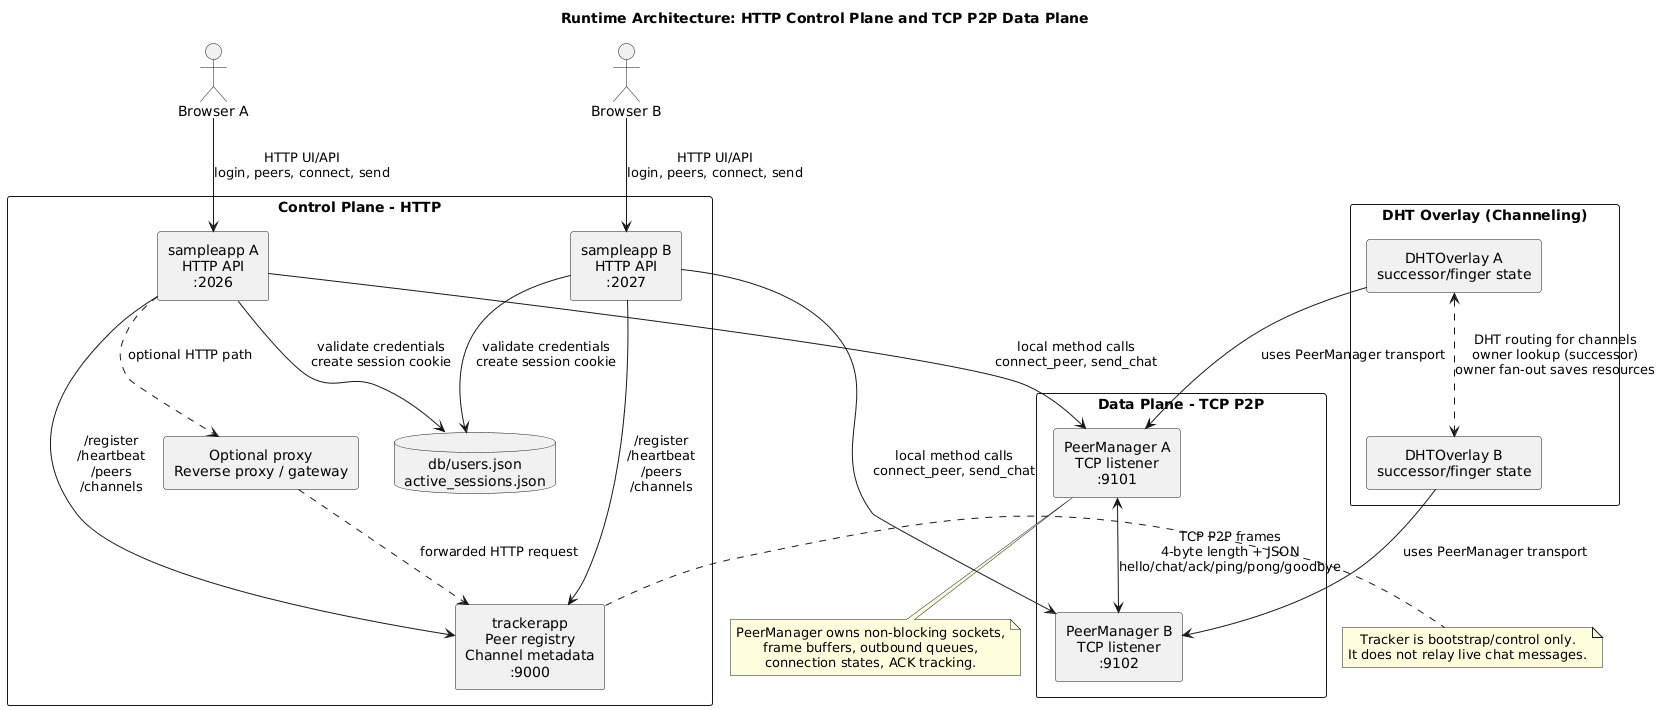
\includegraphics[width=\textwidth]{assets/diagrams/architecture-overview.png}
\caption{Tổng quan kiến trúc runtime của hệ thống}
\end{figure}

\subsection{Architectural boundaries}

Kiến trúc hiện tại có các ranh giới trách nhiệm rõ ràng:
\begin{itemize}[leftmargin=2em]
    \item Browser không giữ kết nối TCP P2P; browser chỉ gọi HTTP API.
    \item Sampleapp không tự relay live message; nó chuyển yêu cầu gửi/nhận xuống PeerManager.
    \item Tracker không chuyển tin nhắn chat trực tiếp; tracker chỉ quản lý bootstrap, active peers và channel metadata.
    \item PeerManager không xử lý login/session; nó chỉ xử lý transport P2P và protocol state.
    \item DHT overlay là tầng routing ở application layer cho channeling/broadcast (phương án nhóm sử dụng để tiết kiệm tài nguyên); transport cuối cùng vẫn là PeerManager.
\end{itemize}

Ranh giới này làm báo cáo và implementation nhất quán: authentication thuộc HTTP control plane, tracker thuộc bootstrap/discovery, còn live chat delivery thuộc TCP P2P data plane.
